% \documentclass[a4paper,9pt,fleqn,notoc]{diss}
% \renewcommand{\includegraphics}[1][1]{}
% \begin{document}

\chapter{Multi-word lexical systems for expressing landmarks}
\label{s:multi-word}
Conceptual alignment is powerful but also has its limits. The most prominent of which
is that conceptual alignment is based on the idea that the population agrees on using a 
single strategy. Now, even a superficial look at English and German reveals that, in fact, 
these languages support many different ways of conceptualizing space at the same time. 
The reason for allowing diverse strategies to flourish in a population is clearly related to 
the ability to discriminate and denote many objects in different spatial settings.
German and English exhibit a rich system of different conceptualization
strategies such as allocentric and egocentric, but they also allow the usage of different frames of reference,
all of which enables agents to be successful in communication particularly when facing different spatial layouts 
and features of the particular environment. The grammar of the respective languages organizes
the expression of these different strategies, but the expression of each strategy also relies heavily on 
lexical systems which go beyond simply expressing the names of spatial relations. 
In this section I consider the expression of compositional semantics using lexical items. 
This is the first step towards grammar and a necessary prerequisite for grammatical development. 

In particular, this section details the step from single-word utterances encompassing only the lexical 
items of spatial categories to multi-word utterances which besides the spatial relation express 
semantic entities as part of the conceptualization strategy. A good example for these are
reference objects which are typically themselves marked using lexical items such as 
in \textit{links von dir} (`to the left of you') which explicitly marks the reference object as being
the hearer via the pronoun \textit{dir} (`you'). Earlier sections of this book already 
dealt with lexical systems and much of the discussion applies to extended lexical systems which 
incorporate lexical items for landmarks and the like. Essentially, one is 
left with generalizing the construction invention and adoption operators for spatial 
categories to include other semantic entities. This endows agents with the capacity for lexical marking 
of reference objects as part of conceptualization strategies. This single step to 
multi-word utterances alone, as is argued in this chapter, allows agents to be 
more adaptive and more successful in communication.

\section{Invention and alignment operators}
%unexpressed-meaning-production
%invent-lexical-items-in-production
%adopt-lexical-items
In order to study the behavior of systems that allow for more expressiveness using 
multi-word utterances, I adapt the operators that invent constructions for spatial categories 
and extend them to deal with semantic items that are not spatial categories. 
Technically, these operators enable speakers to invent constructions for bind statements in the 
conceptualized meaning they want to express. On the other hand, hearers can employ 
similar operators that adopt unknown strings by linking them to bind statements in 
interpreted meaning, specifically in re-conceptualized meaning. 
Figure \ref{f:egocentric-speaker} shows the 
meaning conceptualized for a particular context using an egocentric strategy. The
meaning contains two bind statements, i.e. two semantic entities, for which the agent
has invented two lexical constructions. One for the spatial category and
one for the discourse role {\footnotesize\tt speaker}. Consequently, the speaker
utters two words for this particular meaning. In this case the meaning will be conveyed 
using the utterance \textit{rexute calipo} with no word-order constraints applying. 
In fact, because there are no word order constraints, the strings are shuffled and the speaker 
is equally likely to utter any permutation of the two words. The hearer upon encountering such
an utterance will use the power of re-conceptualization to find an appropriate interpretation
of the utterance which sets up the learning context. Depending on how much he already knows, this might be an easy task. However, if he does not know any of the two words, 
he first has to invent a category based on the topic and the most likely conceptualization 
strategy given the current context.
Let us suppose the hearer has already encountered the spatial category named by the 
word \textit{rexute}. If he re-conceptualizes that the speaker most probably used an egocentric
strategy, the interpreted meaning looks very similar to the meaning conceptualized 
by the speaker; the only difference being that he uses his spatial category. 
Because there is precisely one unknown word for the hearer and one 
bind statement in the interpreted meaning
that is not linked to a word in the utterance, this presents a learning opportunity for the
hearer and he can adopt the word \textit{calipo} to mean the discourse role {\footnotesize\tt speaker}.

\begin{figure}[h]
\begin{center}
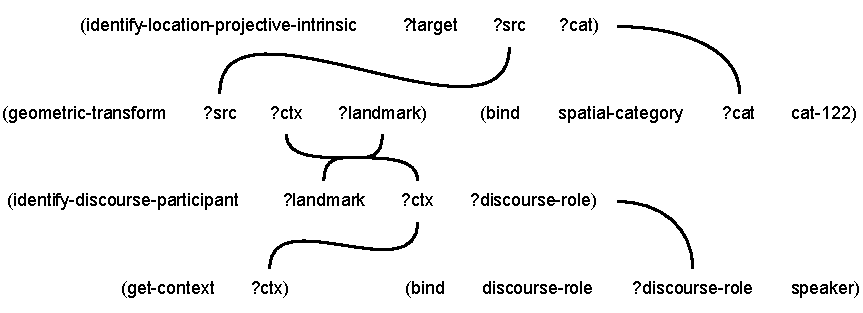
\includegraphics[width=1.0\columnwidth]{figs/semantic-structure-egocentric-speaker}
\end{center}
\caption{Semantic structure for an egocentric conceptualization.}
\label{f:egocentric-speaker}
\end{figure}
\begin{figure}
\begin{center}
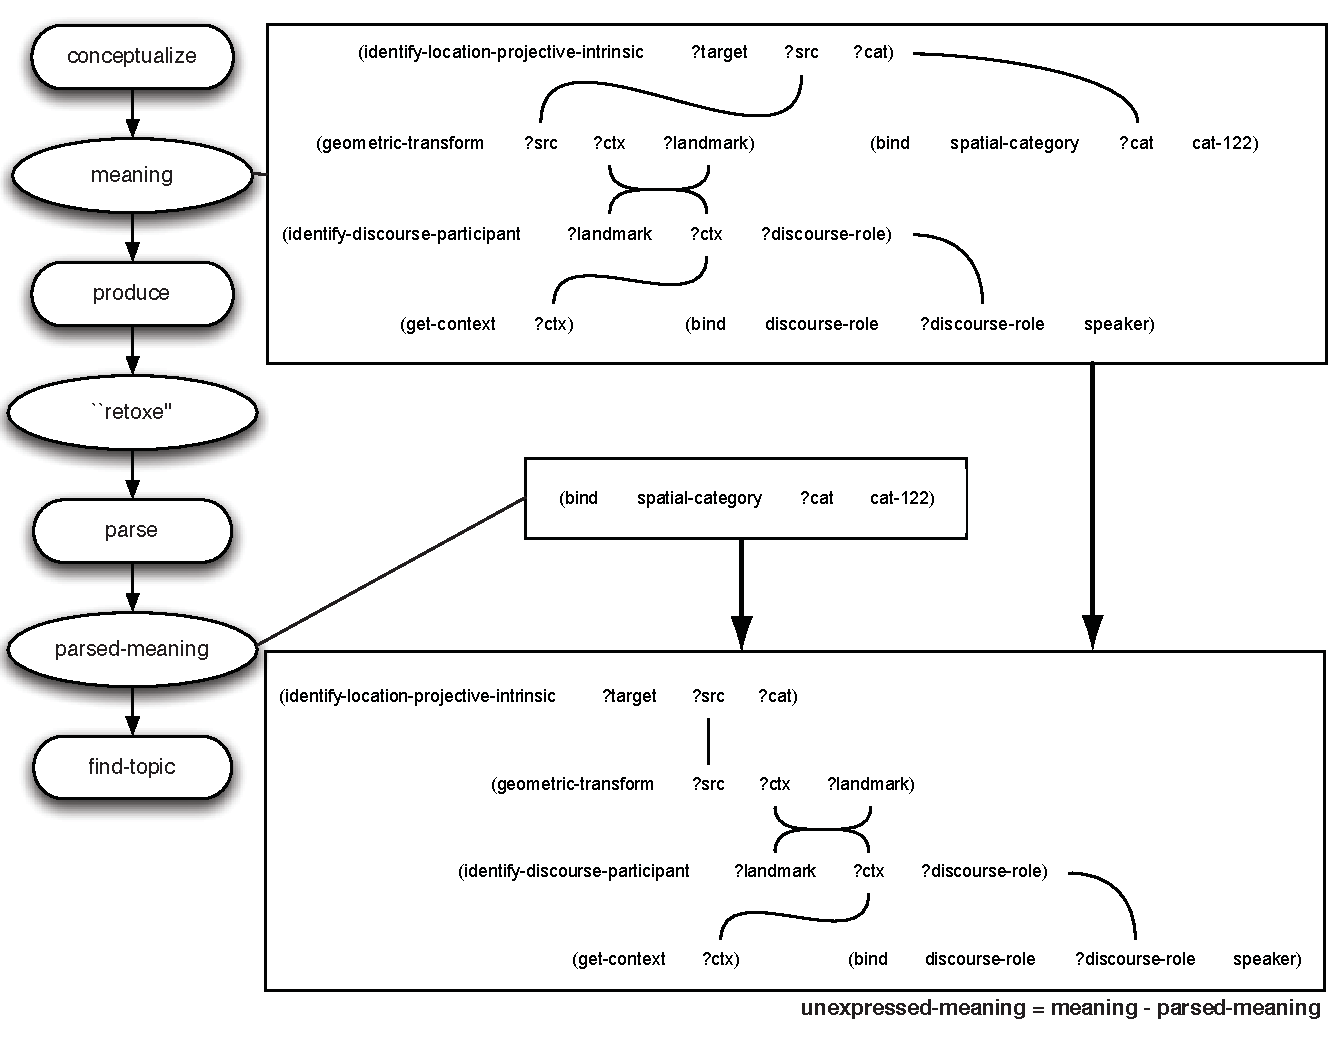
\includegraphics[width=1.0\columnwidth]{figs/mark-unexpressed-meaning}
\end{center}
\caption[Grammatical marker invention]{Example of a learning situation in which agents invent additional names 
for semantic entities in production. The left shows the processes run as 
part of production. Suppose the agent has conceptualized the meaning shown 
on top. He produces for this topic. Because he already has a construction to
express the category {\footnotesize\tt cat-122}, he would utter the word \textit{retoxe}.
Before passing the utterance to the hearer, he re-enters the utterance himself
and interprets the parsed meaning. Having only expressed the category, 
he potentially interprets different target objects.
He detects this problem and extracts the unexpressed meaning shown below which
consists of the complete network without the category which was expressed in
the utterance. A repair strategy can now scan the unexpressed meaning and
potentially invent a lexical construction for the discourse role {\footnotesize\tt speaker}
which was not expressed. The same mechanism is re-used for the evolution of grammatical 
systems discussed in later sections.}
\label{f:marking-unexpressed-meaning}
\end{figure}

There are two types of problems that lead to the invention of new markers. 
First, if production for a particular meaning fails altogether, i.e. no utterance can be 
produced, a specific diagnostic triggers and reports a problem. This problem immediately 
starts a dedicated repair strategy which scans the meaning, looks for bind statements and invents new words for all bind statements in the meaning. Preference is given for inventing words for spatial categories. The reason is that if an agent cannot express a spatial category used in conceptualization, this category has just been invented by him. 
The invention of lexical constructions linking to other semantic entities is controlled by
a parameter that adjusts how eager agents invent new linguistic items.
The second situation that might lead to the invention of new markers is when
agents notice in re-entrance\is{re-entrance} that they might be misunderstood. This is typically
the case if an agent is conceptualizing using a category that already has a name.
In such cases production will use that name which leads to a single-word utterance consisting of the category name. If the agent re-enters, that is parses and interprets his 
own utterance before passing it to the hearer, he might find that the category name
alone does not exclude other conceptualization strategies in interpretation.
Let us suppose an agent has conceptualized the category {\footnotesize\tt cat-122} using
an egocentric strategy. If he only utters the word associated with that category, other
conceptualization strategies such as allocentric and egocentric hearer are possible
and might lead to other interpretations. A special diagnostic identifies this condition
and reports a problem. The repair strategy triggered by these problems will
solves the problem by inventing a marker for the bind statement in the conceptualized 
meaning that the speaker could not recover when parsing his own utterance.
The process of marking unexpressed meaning is important and will play a significant 
role in later sections. Figure \ref{f:marking-unexpressed-meaning} gives an overview of this process.
The hearer uses the same learning operators for diagnosing and repairing the re-production 
process. But instead of inventing new strings, he re-uses unknown strings from the
utterance passed to him by the speaker.

Lexical constructions denoting additional bind statements are subject to the same
alignment control operations as all the other lexical constructions for spatial relations.
However, there is a fundamental difference in the way semantic entities like discourse roles and 
object classes are treated in this book from the way spatial categories are treated. 
The representations of spatial categories are shaped by agents and it is part of the argument
how spatial categories are adapted. For object classes
and discourse roles this does not hold. Rather, 
such entities are given to agents and their internal representation is fixed. 
For these items then the problem of language evolution reduces to mere naming 
problems, i.e. finding words for established concepts. The discussion of how these items, 
i.e.  the agent internal concepts, can emerge and how they are shaped is not discussed 
here. For the emergence of naming systems, however, the same 
insights apply as for the lexical systems involving categories. Lexical constructions for naming such
concepts are subject to continuous tracking of their respective success as well as punishment of competitors
for the same concepts using lateral inhibition. 

Lastly, a hearer encounter a situation where he is confronted 
with two unknown words in
the utterance passed to him by the speaker. While the he might 
nevertheless be able 
to re-conceptualize some meaning involving two semantic entities, 
he faces a tough problem because in principle all possible linkings 
between the two semantic entities and the two words are possible. 
In such cases hearers give up and learn neither of them. 

\section{Experimental setup and results}
I test the effectiveness of the learning operators on spatial scenes. 
The main factor manipulated
is the objects eligible to be topics. The robots and the allocentric landmarks, 
in each scene are also sometimes topics of communicative interactions. 
So instead of just talking about the blocks in their environment
agents now have to talk about themselves and the box landmark. The idea behind this is that 
scenes where the reference objects themselves are chosen as topic help agents develop a system for 
naming these objects. The growing lexical system for reference objects can then be re-used when 
inventing and adopting new spatial categories in conceptualization strategies featuring the reference objects.
In other words, this allows the systems for marking reference objects and spatial categories to co-evolve.

\begin{figure}
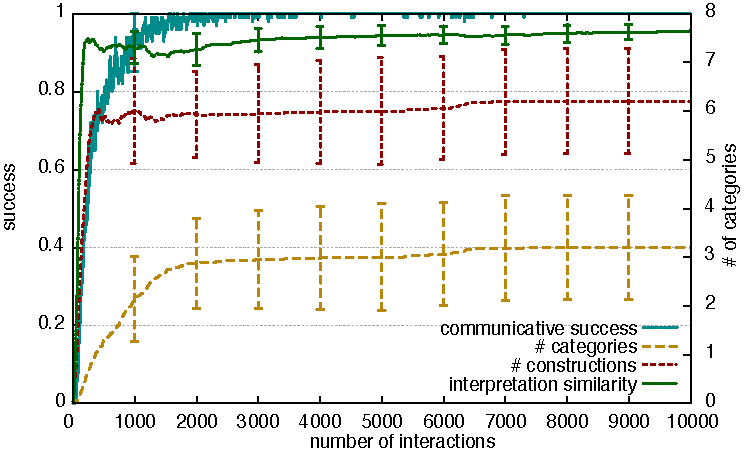
\includegraphics[width=1.0\columnwidth]{figs/chunk-alignment-formation-projective+marking-space-game-5}
\caption[Results strategy competition]{Results for an experiment were agents are equipped with three conceptualization
strategies: allocentric, egocentric speaker and egocentric hearer. Additionally, agents are given
invention and adoption mechanisms for lexical constructions to denote the landmarks themselves.}
\label{f:marker+category-formation}
\end{figure}

Figure \ref{f:marker+category-formation} shows that lexical learning operators 
extend well to semantic entities that are not 
spatial categories. Agents in the experiments summarized in the graph are 
equipped with 
allocentric and egocentric projective strategies (intrinsic). We can see that agents not only 
develop categories but also lexical items to name the three possible reference objects. 
We can see that agents reach success fast with synonyms arising for the different
reference objects that are gradually removed again from the population. The number of constructions\is{measures!number of constructions}
stays consistently higher than the number of categories\is{measures!number of categories} which refers to the lexical constructions 
that link to object classes and discourse roles. In total, agents need three additional constructions -- one for each strategy.

One can contrast these results to some extent 
with alignment of conceptualization strategy results.
Figure \ref{f:alignment-vs-marking} compares the 
communicative success\is{measures!communicative success} and shows that for all things
being equal, allowing agents to mark the 
conceptualization strategy is overall more successful
and reaches successful levels faster than relying on 
only on alignment of conceptualization strategies.
Such comparisons, however, have to be read very carefully. 
First, the dynamics of alignment is
subject to sets of parameters and sometimes small 
changes in these parameters have significant 
effects on overall communicative success\is{measures!communicative success}, but also 
on the dynamics of development. Second,
the experiment shows one particular run in a particular environment. Nevertheless, it seems
reasonable to extrapolate these results. If agents have the capacity to be more expressive, this clearly helps them in being more precise in communication. 
In particular, the expression of reference objects eliminates the major 
source of errors in conceptualization alignment\is{alignment}, 
namely the problem of guessing the strategy used. It is therefore plausible to assume that
marking always outperforms strategy alignment\is{alignment} in sufficiently complicated environmental conditions
that necessitate the balancing of different strategies.


\begin{figure}
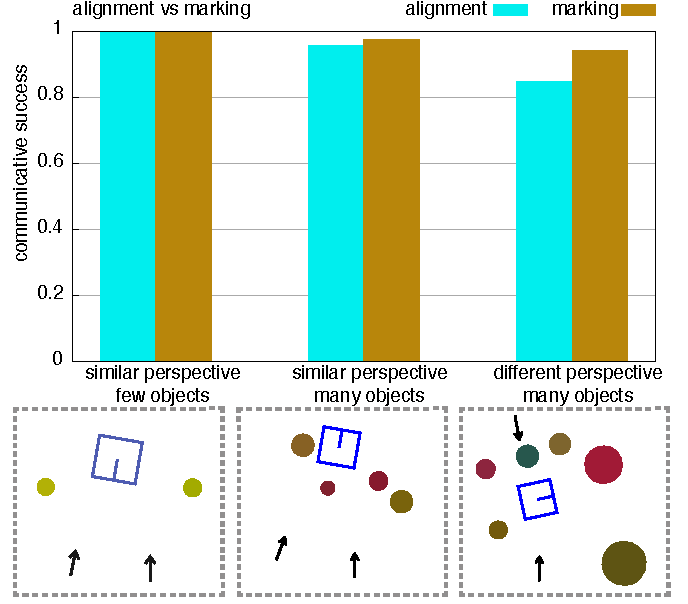
\includegraphics[width=1.0\columnwidth]{figs/chunk-alignment-vs-marking-space-game-5--11}
\caption[Comparison of alignment versus lexical 
marking of strategies]{Comparison of alignment only versus lexical 
marking of strategies. The results are based on landmark selection 
and three strategies are available to agents: allocentric, 
speaker and hearer. In the ``alignment'' condition agents 
are given the three strategies plus mechanisms for strategy alignment. 
In the ``marking'' condition
agents can develop a lexicon for disambiguating the strategy 
they are using in a particular language game. The two approaches 
are tested on different sets of spatial scenes.
The more complex spatial scenes are, the larger is
the advantage of marking the conceptualization
strategy.}
\label{f:alignment-vs-marking}
\end{figure}
 
\section{Discussion}
% lexical marking is not everything
One can conclude that lexical expressivity is enormously 
helpful and allows agents to develop 
communication systems more rapidly and more successfully. 
Additionally agents can be successful in different environments 
and spatial setups, because the different conceptualization
strategies co-exist at the same time and there is no need for 
competition and alignment of strategies 
in the strict sense. Lexical marking, consequently, also leads to 
more adaptive systems if the environment
changes later. All it takes, if new possible reference objects 
arise, is to invent new markers, whereas
in conceptual alignment agents have to come up with new strategies altogether. 


Lexical-only systems have an additional 
problem with respect to spatial language. 
Lexical marking cannot disambiguate semantic 
structure that encompasses the same semantic 
entities but different operations. For instance, the utterance 
\textit{der linke block} (`the left block') has a different semantic
structure than \textit{links des blockes} (`to the left of the block'). 
Albeit both have the same lexical items, there is a clear difference 
in semantic function. In the case of the adjective noun phrase, 
\textit{links} (`left') is used as a modifier modifying the set of blocks. 
In the case of the prepositional phrase \textit{links} (`left') is related to a 
landmark denoted by the determined noun phrase \textit{des blockes} (`the block'). 

More information can be found in \citealt{spranger2012stages,spranger2013evolutionary}.\index{Spranger, M.}

% \end{document}